\documentclass{sig-alternate}
\begin{document}
\title{Convolutional Layer Normalization}
\numberofauthors{4} 
\author{
\alignauthor
Zichao Li\\
    \affaddr{The Chinese University of Hong Kong}\\
    \affaddr{1155081754}\\
    \email{zcli@cse.cuhk.edu.hk}\\
\alignauthor
Junpeng Ye\\
    \affaddr{The Chinese University of Hong Kong}\\
    \affaddr{1155086759}\\
    \email{jpye@cse.cuhk.edu.hk}\\
\and
\alignauthor
Yinpeng Guo\\
    \affaddr{The Chinese University of Hong Kong}\\
    \affaddr{1155081867}\\
    \email{ypguo@cse.cuhk.edu.hk}\\
\alignauthor
Hongchen Li\\
    \affaddr{The Chinese University of Hong Kong}\\
    \affaddr{1155081817}\\
    \email{lihc@cse.cuhk.edu.hk}\\
}
\maketitle
\begin{abstract}
Gradient vanishing is always one of the major difficulties when training state-of-the-art neural network. Among various techniques that deal with this problem, batch normalization and layer normalization are the most popular ones because of their simplicity and effectiveness. However, both of them have drawbacks. Batch normalization is not suitable for online learning and layer normalization performs relatively poor when applied to convolutional neural networks. In this report, we propose a new normalization techniques called convolutional layer normalization that tackle these shortcomings. Compared to batch normalization and layer normalization respectively, convolutional layer normalization is not sensitive to the minibatch size and more suitable for the convolutional neural network. We conduct the experiment on CIFAR-10 datasets and compare the result with batch normalization and layer normalization. The experiment result demonstrates that with small mini batch size, convolutional layer normalization outperforms the batch normalization and layer normalization. Our main contribution is scale the layer normalization to the convolutional layers and make normalization techniques suitable in online learning situtaion. 

\end{abstract}

\keywords {Deep Learning; Optimization; Convolutional Neural Network;}

\section{Introduction}
    A range of successful applications using Deep Neural Network (DNN) in recent years has proved that DNN is a better choice when tackling various difficult problems. Among numerous applications in different fields of DNN, Computer Vision (CV) draws the most attention. CV become one of the best application scenes for DNN since Alex Krizhevsky proposed AlexNet in 2012 \cite{krizhevsky2012imagenet}. Various research were carried out after that, including real-time object detection \cite{ren2015faster}, image captioning \cite{vinyals2015show}, face verification \cite{taigman2014deepface}, image generation \cite{gregor2015draw} and many others. Deep learning has become a game changer in CV. Typically, the convolutional neural network is proven to be quite powerful in CV. Now, the state-of-the-art DNN models can achieve equivalent or even better performance than human in image classification tasks.

    One obvious trend of deep learning is that the network goes deeper and deeper. As a comparison, AlexNet has eight layers and achieved 16.4\% in the ImageNet classification top 5 error while ResNet \cite{he2015deep} has 152 layers and achieved 3.57\% in top 5 error. It is reasonable that the deeper network performs better than the shallower network. It is intuitive to deepen the network because as 
    the architecture goes deep, the model will have more learnable parameters and introduce more non-linearity. As a result, the model can learn more complex data. However, more parameters and non-linearity also requires more computing power and it is more difficult to train.

    Having always been one of the most awkward obstacles in DNN, gradient vanishing slows down training rate of DNN as well as development for more powerful industrial applications. To wipe out this obstacle, a number of researches have been conducted, like careful weight initialization \cite{sutskever2013importance}, careful activation function selection \cite{he2015delving}. Among which Batch Normalization \cite{ioffe2015batch}, Layer Normalization \cite{ba2016layer} and Weight Normalization \cite{salimans2016weight} are the most popular. 

    Batch normalization uses the distribution of the summed input to a neuron over a mini-batch of training cases to compute a mean and variance which are then used to normalize the summed input to that neuron on each training case. This significantly reduces the training time in feedforward neural networks. However, the effect of batch normalization is dependent on the mini-batch size, which is not suitable for Online Learning. Besides, it is not obvious how to apply it to recurrent neural networks. On the other hand, another method called Layer Normalization is flexible for Online Learning, but it performs poorly on Convolutional Neural Network. In terms of this problem, we propose a more general version of Layer Normalization, which is called Convolutional Layer Normalization. It is robust to the input data, weight initialization, and the form of the activation function. In addition, it has no limit on the network architectural and batch size.


\section{Related Work}

    \begin{figure}[t!]
        \centering
        \centerline{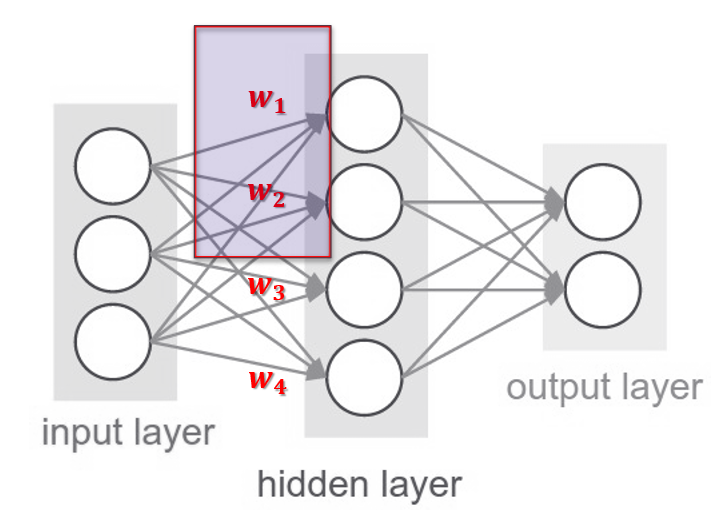
\includegraphics[width=8cm]{batch_norm}}
        \caption{Batch Normalization}
        \label{fig:batch_norm}
    \end{figure}
    \begin{figure}[t!]
        \centering
        \centerline{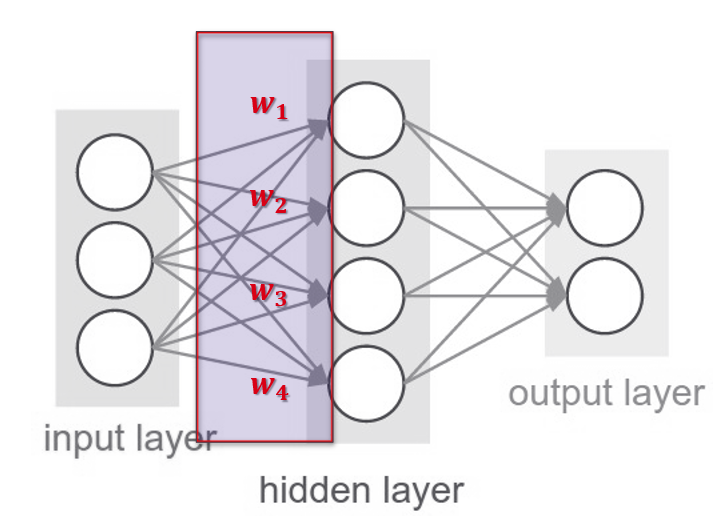
\includegraphics[width=8cm]{layer_norm}}
        \caption{Layer Normalization}
        \label{fig:layer_norm}
    \end{figure}
    
    Some related works to our method are Batch Normalization, Layer Normalization, and Weight Normalization, among which the former two methods should be taken into account more attentively.
    Batch Normalization is a significant algorithm in response to reducing neural networks’ dependency on parameter initialization by means of normalizing each input for each mini-batch with the simple statistics (0 mean and 1 variance) of certain mini-batch, meanwhile accelerating the learning rate in contrast to traditional networks. 
    Nonetheless, there is still an obvious drawback of this method that if the size of mini-batch is too small, the sampling error would make the Batch Normalization perform poorly. This problem can not be resolved due to the inborn feature of Batch Normalization.
    In order to deal with the problem mentioned above, a new method called Layer Normalization is proposed. It considers normalization in a different perspective that to normalize the inputs within each layer rather than within each mini-batch. This improvement is very meaningful because it frees limitation of the size of mini-batch. However, it has a significant assumption that each neuron contributes equally to next layer, which is far away from truth in Convolutional Neural Network.
    Besides, there is another normalization method called Weight Normalization, an approach to weights reparameterization which achieved ** in** field. It is closely related to Batch Normalization that in some special case, e.g. , it can be regarded as equivalent to Batch Normalization. However, our method is not kind of reparameterization. Instead, it is invariance under different parameterization of weights, so it is more robust.
\section{Fisher Modules for Layer Normalization}
    \subsection{Layer Normalization for Convolutional Layer}
    Given the special architecture of CNN, we need to find a way to measure the contribution of each unit within the same layer to the final output. Fisher Information Matrix is used in Natural Gradient to measure how the distribution of final output would change with the change of parameters, i.e, 
    \begin{displaymath}\pmb{F}(w)=E[\frac{\partial\log p(\pmb{w,x})}{\partial w_i}\frac{\partial\log p(\pmb{w,x})}{\partial w_j}] 
    \end{displaymath}
    In the normalization case, we want to measure the change of output with respect to the each unit. And we also need to adapt the FIM to neural network. For unit $k_n, k_m$ in output layer $l_{out}$, the associated entry of the FIM should be:
    \begin{equation}
        \pmb{F}_{k_nk_n} = E[\frac{\partial\log p(y)}{\partial a_{k_n}}\frac{\partial\log p(y)}{\partial a_{k_m}}]
    \end{equation}
    Thus the norm $||\delta y||$ of the probability distribution of output is 
    \begin{equation}
        ||\delta y|| = \sum_i\sum_j\sum_{k_n}\sum_{k_m}E[\frac{\partial\log p(y)}{\partial a_{k_n}}\frac{\partial\log p(y)}{\partial a_{k_m}}\delta a_i\delta a_j]
    \end{equation}
    where $a_{k_n}$ denotes the output of unit $k_n$.
    It is easy to scale the entry to each hidden unit through back propagation$\frac{\partial a_k}{\partial a_i}=\beta_i^{k}$.
    where $\beta_i^{k}$ is the back propagation rate\cite{LeCun1998}
    Set $\beta_{k_n}^{k_n}:=1$ for $k_n$ in the output layer and $\beta_{k_m}^{k_m}:=0$. Let one output unit $k_n$ equals to 1 and others equals to 0, 
    \begin{equation}
        \beta_{i}^{k_n} = \sum_{j, i\rightarrow j}w_{ij}\nabla a_j \beta_j^{k_n} 
    \end{equation}
    where $\nabla a_j$ is the gradient of the activation function in unit $a_j$. It can be regarded as a unit of back propagation value, thus the name. 
    (2) can be futher extended to:
    \begin{equation}
        ||\delta y|| = \sum_i\sum_j\sum_{k_n}\sum_{k_m}\pmb{F}_{k_nk_m}\beta_i^{k_n}\beta_j^{k_m}
    \end{equation}
    $\pmb{F}_{k_nk_m}$ varies in different activation functions of output layer. And consequently the resulting block of $\pmb{F}_{i,j}$ is distinctive:
    \begin{enumerate}
        \item For the sigmoid function
        \begin{equation}
            \pmb{F}_{i,j} = \sum_{k}\frac{\beta_i^{k_m}\beta_j^{k_m}}{a_{k_m}(1-a_{k_m})}
        \end{equation}
        \item For the softmax function
        \begin{equation}
            \begin{aligned}
            \pmb{F}_{i,j} = \frac{1}{\sum_k e^{a_{k_m}}}\sum_k [e^{a_{k_m}}\beta_i^{k_m}\beta_j^{k_m}]
            \\
            -(\frac{1}{\sum_k e^{a_{k_m}}})^{2}(\sum_k e^{a_{k_m}}\beta_i^{k_m}\beta_j^{k_m})
            \end{aligned}
        \end{equation}
        \item For the linear mapping
        \begin{equation}
            \pmb{F}_{i,j} = \sum_k \beta_i^{k_m}\beta_j^{k_n}
        \end{equation}
    \end{enumerate}
    If we assume the units within same layer is independent of each other, only the block diagonal entries of the FIM is needed. Then only $\pmb{F}_{i,i}$ is taken into account. Define $\Phi_i(x) \equiv \pmb{F}_{i, i}$. For instance, for the classification task, which is included in our experiment later
    \begin{equation}
        \begin{aligned}
         \Phi_i(x)= \frac{1}{\sum_k e^{a_{k_m}}}\sum_k [e^{a_{k_m}}(\beta_i^{k_m})^{2}]\\
         -(\frac{1}{\sum_k e^{a_{k_m}}})^{2}(\sum_k e^{a_{k_m}}\beta_i^{k_m})^{2}
        \end{aligned}
    \end{equation}
    These conclusions are mostly derived by \cite{DBLP:journals/corr/abs-1303-0818}. It is intuitive to follow this approach to measure the contribution of each hidden unit to the final output. But it is nearly impossible to measure $\Phi_i(x)$ accurately. First of all, the computational cost of back propagation rate $\Phi_i(x)$ is proportional to number of output units. If there are $n$ output units, it takes $n$ times to calculate all the $\beta_i^{k_m}$ for a certain unit. The computational cost is $O(n_{output}n_{input})$, which is huge.  Besides, the value of $w$ and $\nabla a$ changes in each iteration, it means that it takes double time to compute the fisher modules. 
    
    Recall the original Fisher Modules $\Phi_i(x)$ is the contribution of unit $i$ for a certain input $x$, but what we need here is another method to compute the expectation value of $\Phi_i(x)$ with expect to $y, w, x, \nabla a$. Assume an informative prior over the final output, i.e., $a_k = 1/n_{class}$. Or it can be set by the output class distribution in training set. For $\nabla a$, we can directly calculate the expectation value in the following way:
    \begin{enumerate}
        \item For Relu activation:
            \begin{equation}
            E\nabla a_i = \frac{1}{2} \times 0 + \frac{1}{2} \times 1 = \frac{1}{2}
            \end{equation}
        
        \item For Sigmoid function, we assume the input value $a_{i^{'}}$ of a unit is over a Gaussian distribution with mean $\mu$ and variance $\sigma$. Then 
            \begin{equation}
                \begin{aligned}
                E\nabla a_i = \nabla Ea_i\\
                = \nabla\int_{-\infty}^{\infty}\frac{1}{1+e^{-a_{i^{'}}}}\mathcal{N}(a_{i^{'}}|\mu, \sigma)da_{i^{'}}
                \end{aligned}
            \end{equation}
            Approximate the Sigmoid function by the cumulative distribution function, thus
            \begin{equation}
                \begin{aligned}
                Ea_i \approx \int_{-\infty}^{\infty}F_{a_{i^{'}}}(\lambda a_{i^{'}})\mathcal{N}(a_{i^{'}}|\mu, \sigma)a_{i^{'}}\\
                = F_{a_i}(\frac{\lambda\mu}{\sqrt{1+\lambda^{2}\sigma}})
                \end{aligned}
            \end{equation}
            When $\lambda$ equals to 0.588, $F_{a_i}(\lambda a_i)$ fits the Sigmoid function best. Recall that the input units within the same layer are normalized to a 0 mean and 1 variance distribution. As a result, $\mu = 0$ and $\sigma = 0.01$, then $Ea_i$ = 0.5, and
            \begin{equation}
                \begin{aligned}
                    E\nabla a_i = a_i(1-a_i) = 0.25
                \end{aligned}
            \end{equation}
        \item For Softmax activation, the derivation is similar to the one of Sigmoid function, thus:
            \begin{equation}
                \begin{aligned}
                E\nabla a_i = p_m(1-p_m)\\ = \frac{1}{n_{class}}(1-\frac{1}{n_{class}})
                \end{aligned}
            \end{equation}
            where 
            \begin{equation}
                p_m = \frac{e^{a_{k_m}}}{\sum_ke^{a_k}}
            \end{equation}

    \end{enumerate}
    As for the parameter $w$, there are two approaches, one is to use a moving average. In the first iteration, $w$ is initialized with Gaussian distribution with 0 mean and 0.01 variance. Other initialization techniques are also available. And then after each $n$ iterations, the parameter $w$ is updated once with a decay parameter $t$. Here is a trade-off, between the accuracy of the real value of $w$ and the saving of computational effort. The other one is more like a trick. We just set all the $w$ in layer $l$ equals to $1/n_{l-1\rightarrow i}$, where $n_{l-1\rightarrow i}$ denotes number of the units connected to the unit $i$ in incoming layer $l-1$. The simple intuition behind is we assume the contribution of every units connecting to the same unit is equal. And according to our experiment, this approach works pretty well, and it nearly has the same performance to approach one. In the experiment section, the implementation of our normalization methods is in this approach. 
    
    The Fisher modules itself can be further approximated. If all the terms of $\beta_i^{k_m}\beta_i^{k_n}$ are neglected, then the Fisher Modules, for instance, under the classification task, (8) can be simplified to
    \begin{equation}
        \begin{aligned}
         \Phi_i(x)= \frac{1}{\sum_k e^{a_{k_m}}}(\sum_k e^{a_{k_m}}\beta_i^{k_m})^{2}\\
         -(\frac{1}{\sum_k e^{a_{k_m}}})^{2}(\sum_k e^{a_{k_m}}\beta_i^{k_m})^{2}\\
         = (\frac{1}{n_{class}} - \frac{1}{n_{class}^{2}})\sum_k\beta_i^{k_m} 
        \end{aligned}
    \end{equation}
    Consequently, the back propagation rate could be calculated simultaneously. With the second approach of measuring $w$, the computational complexity of approximated Fisher Modules is then $O(1)$. 
    Indeed in the shallow networks, the terms of $\beta_i^{k_m}\beta_i^{k_n}$ can be eliminated. But in the networks with many layers, thoese terms also plays significant role in the Fisher Modules. Hence, them can not be calculated at the same time. But in most networks with two or more hidden layers in the final blocks, for a certain unit $i$, $\beta_i^{k_m}$ should be equal running over all the $k$. Thus, the back propagated rate can be calculated once with arbitrary output units fixed and plugged it into (8). 
    
    After finished calculating with the statics above, the approximated fisher modules can be used as a weight $e^{\Phi_i}$ to measure the mean and variance.
    
    The full algorithm is shown in following Algorithm \ref{alg:gradiantdescent}.

    \begin{algorithm}
        \caption{Convolutional Layer Normalization}\label{alg:gradiantdescent}
        \begin {algorithmic}[1]
            \STATE \textbf{Initialize} $w_l$
            \STATE \texttt{Assign $n_{int}$}
            \STATE $\beta_k_n^{k_n} \rightarrow 1$
            \FOR{$i$ in $l$}
                \STATE \texttt{$\beta_{i}^{k_n} \leftarrow \sum_{j, i\rightarrow j}w_{ij}\nabla a_j \beta_j^{k_n}$}
                \STATE \texttt{Calculate $\Phi_{i}$}
            \ENDFOR
            \STATE \texttt{$\mu_l \leftarrow \frac{1}{n_{l}}\sum_i \frac{e^{\Phi_i}}{\sum_i e^{\Phi_i}}a_{i^{'}}$}
            \STATE \texttt{$\sigma_l \leftarrow \frac{1}{n_l}\sum_i (a_{i^{'}}-\mu_l)^{2}$}
            \STATE \texttt{$a_{i^{'}}\leftarrow \frac{a_{i^{'}}-\mu_l}{\sqrt{\sigma_l+\epsilon}}$}
            \STATE \texttt{$a_l \leftarrow \gamma a_{i^{'}} + \alpha$}
            \WHILE{$iter \mod n_{int} == 0$}
                \STATE \texttt{$w_l = \lambda w_{l_{old}} + (1-\lambda)w_l$}
            \ENDWHILE
            
        \end{algorithmic}
        
    \end{algorithm}

\section{Experiment Results}
    In this section, we have done experiments in two datasets, one is Mnist and and the other is Cifar-10. We not only simply measure the accuracy and cross entropy, but also try to find out how the approximated accuracy of Fisher Modules influence the final result in Covolutional Layer Normalization and compare robustness to batch size of three normalization methods. In both experiments, Batch Normalization and Layer normalization are baselines. 
    \subsection{Mnist classification}
    
    \begin{figure}[t!]
        \centering
        \centerline{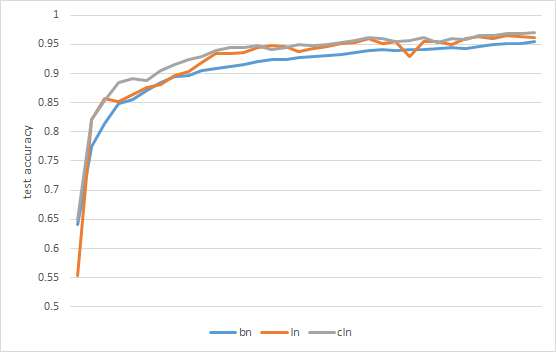
\includegraphics[width=8cm]{accuracy1}}
        \caption{Test Accuracy with batch size 5}
        \label{fig:mnist_acc1}
    \end{figure}
    \begin{figure}[t!]
        \centering
        \centerline{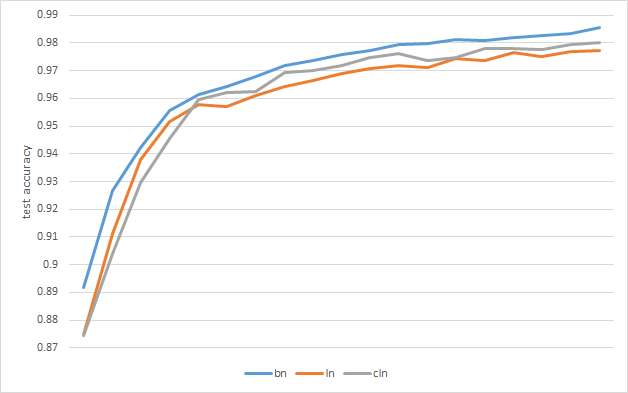
\includegraphics[width=8cm]{accuracy2}}
        \caption{Test Accuracy with batch size 50}
        \label{fig:mnist_acc2}
    \end{figure}
    
    MNIST is a simple computer vision dataset. It consists of images of handwritten digits. The MNIST database of handwritten digits, has a training set of 60,000 examples, and a test set of 10,000 examples. The digits have been  size-normalized and centered in a fixed-size image. Each image is 28 pixels by 28 pixels. No preprocessing is needed and done. It is a 10 class classification task.
    In this experiment, we implement a neural network with three convolutional layers, each followed by a 2x2 max pooling layers. After that there are two fully connected layers. The detailed statistics of the network is in \ref{fig:mnist_acc1} and \ref{fig:mnist_acc2}. We have tried two batch size, 5 and 50 respectively. Theoretically, batch normalization takes more advantage from a bigger batch size. And the experiment result proves it. There is held out test set of 1000 samples, and after each 50 iteration, the trained model is used to measure the accuracy of test set. In this experiment, we measured the back propagation rate $\beta_i^{k_m})$ by (8), i.e., the more accurate way. And the weight parameter $w$ is measure according to the number of fan in units, as mentioned above. 
    
    When the batch size is 50, the Batch normalization still has the highest performance, and the Convolutional Layer Normalization has better performance than Layer Normalization. Since Batch Normalization normalize each unit, it avoids the problem of unit-output relationship calculation. Convolutional Layer Normalization has a solution but it is approximated. When the batch size is big enough, the drawback of depencies in batch size still can be eliminated to less effect than the inaccurate measurement of Fisher Modules. 
    
    However, when the batch size is 5, Convolutional Layer Normalization has test accuracy, and the performance of Batch Normalization decrease rapidly, which proves our assumption that the batch size has high influence on Batch Normalization.


    \begin{figure}[t!]
        \centering
        \centerline{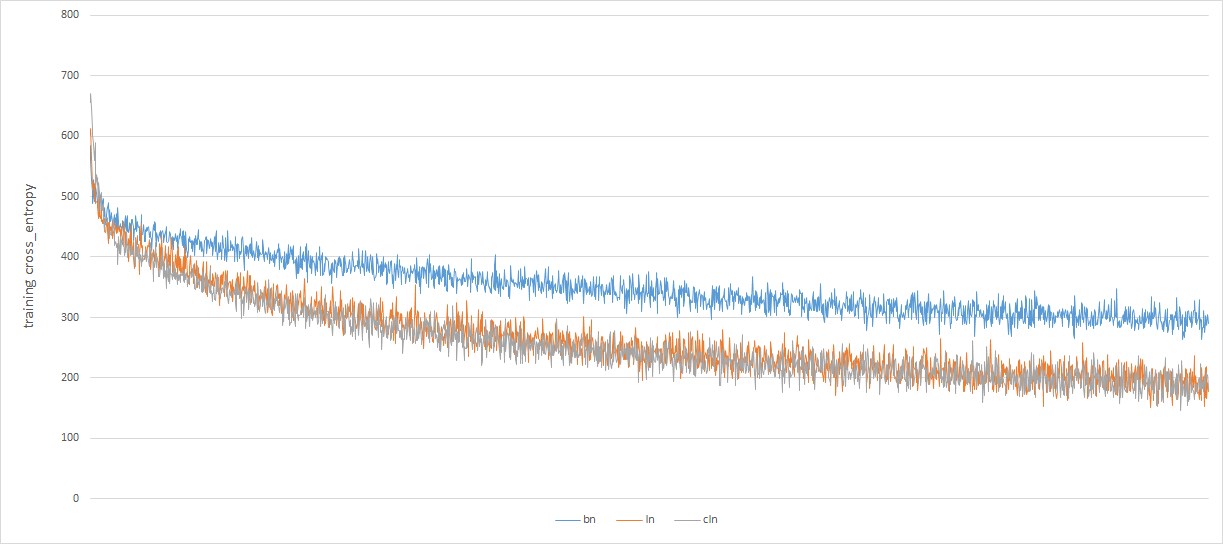
\includegraphics[width=8cm]{loss_clfar}}
        \caption{Cross-Entropy comparision}
        \label{fig:loss_clfar}
    \end{figure}
    
    \subsection{Cifar-10 classification}
    The CIFAR-10 dataset consists of 60000 32x32 colour images in 10 classes, with 6000 images per class. There are 50000 training images and 10000 test images.
    In the preprocessing procedure, we have done some data augmentation, such as random lightness, random flipping left or right, random brightness and Gaussian Noise. We also resize the image to 64x64 so that we can put more max pooling layers. Because of the time and computational resource limit, in this experiment, we just test the case when batch size equals to 5. But other than a more accurate method to measure the Fisher Modules, we use a more coarse grain method(15) to calculate them. Our main target is to see how the accuracy of the Fisher Modules affect the final result. And the cross entropy with respect to the iteration is shown in \ref{fig:loss_clfar}, the Convolutional Layer Normalization still has the best performance. But compared to the Layer Normalization, the difference is quite small. As expected, Batch Normalization is still influenced badly because of the limit of batch size. 

\section{Conclusion and Further Work}
    In this project, we propose a new normalization algorithm, Convolutional Layer Normalizaton, to tackle the problem of gradient vanishing. It measures the contribution of a unit to the distribution of final output a relative principled way to 
\bibliographystyle{abbrv}
\bibliography{sigproc} 

\section{Sample Algo}
Algorithms can be included using the commands as shown in algorithm \ref{alg:gradiantdescent}.

    \begin{algorithm}
        \caption{Gradiant Descent}\label{alg:gradiantdescent}
        \begin {algorithmic}[1]
            \STATE \textbf{Initialize} $\omega$
            \STATE \textbf{Assign} $MaxSteps, \eta$
            \WHILE{$steps\leq=MaxSteps$}
                \STATE {Calculate gradient $\frac{\partial Loss} {\partial \omega}$}
                \STATE {Update parameters: $\omega ^{steps+1} \gets \omega^{steps} + \eta * \frac{\partial Loss} {\partial \omega}$}
            \ENDWHILE
            \STATE \textbf{return} $\omega$
        \end{algorithmic}
    \end{algorithm}
    
\end{document}